\documentclass[12pt, letterpaper]{book}
\usepackage{graphicx} %LaTeX package to import graphics
\graphicspath{{../Immagini}} %configuring the graphicx package

%Domande:
%1) nei dispositivi che stiamo studiando il body è cortocircuitato con il source? 

\begin{document}


\section{La tensione di soglia $V_{th}$}

\paragraph{}
La tensione di soglia $V_{th}$ di un transistore MOS è definita come quella tensione tra gate e bulk per la quale la popolazione di minoritari all’interfaccia è uguale alla popolazione di maggioritari nel bulk. Questa definizione non può essere usata direttamente per il calcolo della tensione di soglia dei dispositivi, ma si deve passare attraverso l'analisi delle misurazioni sperimentali di altri valori, a seconda del metodo utilizzato. \\	
Per lo studio della $V_{th}$ sono stati presi in consifderazione vari metodi, in modo da confrontare i risultati di ciascuno e scegliere quale effettivamente usare per lo studio della degradazione delle prestazioni statiche del chip.\\
Il primo metodo utilizzato è  ottiene la misura della $V_{th}$ attraverso l'analisi della caratteristica $I_D$-$V_{GS}$. Questo grafico presenta un punto di flesso attorno al quale il grafico è linearizzabile. Tracciando il fit lineare nell'introno del punto di flesso si ottiene un retta che interseca l'asse delle ascisse, ovvero quello di $V_{GS}$ in un punto il cui valore corrisponde a quello della $V_{th}$.\\


\begin{figure}[h]
\centering
 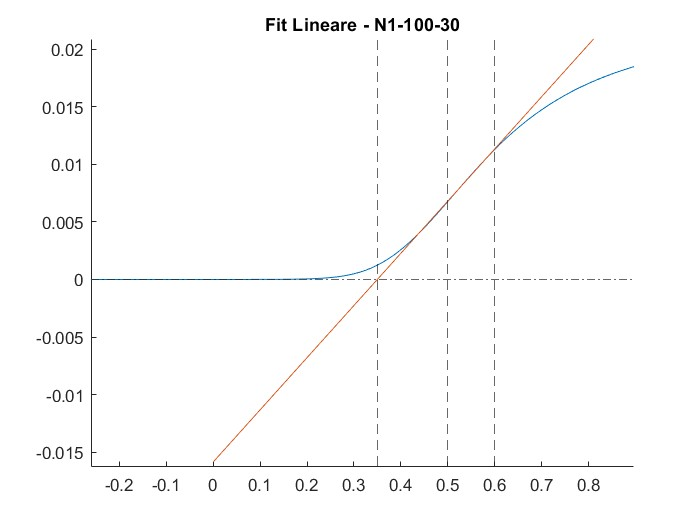
\includegraphics[width=0.45\textwidth]{LinearFit-N1-100-30}
 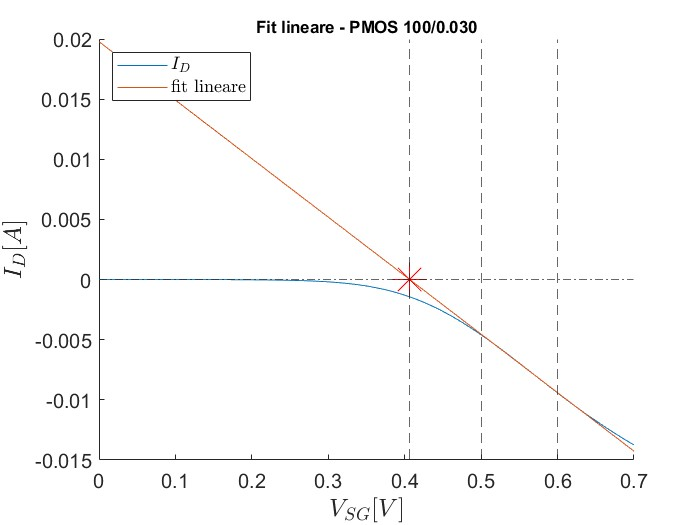
\includegraphics[width=0.45\textwidth]{LinearFit-P1-100-30}
 \caption{Fit lineare della caratteristica  $I_D$-$V_{GS}$ a $V_{DS}=150mV$ di un NMOS e di un PMOS di dimensioni 100-30 nell'intorno $[0,4V ; 0,6V]$ di $V_{GS}$}
\label{fig:scimmia}
\end{figure}


Il secondo metodo utilizzato è chiamato \emph{Transconductance Change Method (TCM)}, che difiscisce la tensione di soglia come la tensione di gate $V_{GS}$ corrispondente al picco massimo della derivata della transconduttanza $g_m$ rispetto alla tensione di gate ed è valido per bassi valori della tensione $V_{DS}$. Questa definizione si basa sul fatto che quando la $V_{GS}$ è pari alla somma tra la $V_{th}$ per come è stata definita all'inizio del capitolo e la $V_{DS}$, i dispositivi passano dalla regione di triodo alla regione di saturazione e, di conseguenza, la caratteristica $I_D$ - $V_{GS}$ passa da un andamento quatratico ad uno lineare quasi costante. \\
La transconduttanza non è altro che la derivata prima della corrente $I_D$ rispetto alla tensione $V_{GS}$, che quindi avrà il suo massimo nel punto corrispondente alla tensione per la qualei il grafico della corrente passa dalla forza quadratrica a quella lineare, ovvero la tensione $V_{GS}+V_{DS}$. Se $V_{DS}$ è piccolo, la tensione per la quale la $g_m$ è massima è molto simile a $V_{th}$.








\end{document}